\begin{python}
    self.dashboard <= w.label('Buttons', typo='headline4', style=flex_title)
    self.dashboard <= w.button(
        'Button 1',
        style=flex,
        on_click=lambda: setattr(
            document.select_one('#for_button'), 'html', 'Button 1 pressed!'
        ),
    )
    self.dashboard <= w.button(
        'Button 2', style=flex, on_click=self.on_button2
    )
    self.dashboard <= w.label(
        f'', id='for_button', typo=f'body1', style=flex
    )

def on_button2(self):
    document.select_one('#for_button').html = 'Button 2 pressed!'
\end{python}


\begin{figure}[H]
\begin{centering}
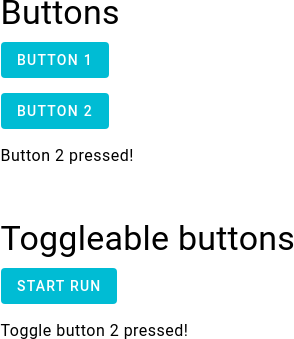
\includegraphics[scale=0.5, left]{Cap4/Figures/widgets/buttons.png}
\par\end{centering}
\caption[Brython Radiant: Buttons]{Brython Radiant: Buttons.}
\label{fig:radiant_buttons}
\end{figure}